\documentclass[11pt, a4paper]{article}
\usepackage{titlesec}
\titlespacing*{\section}{0pt}{0.8\baselineskip}{\baselineskip}
\usepackage{xcolor}
\usepackage{lipsum}
\usepackage{setspace}
\usepackage{float}
\usepackage{graphicx}
\usepackage[justification=centering]{caption}
\renewcommand{\baselinestretch}{1.0} 
\title{A Personalized Photo Enhancement Agent}
\author{Mugdha Jain, Ling Ouyang, Jason Tellis
%make sure to specify if the project is Programming or %Technology Driven
\thanks{CS256 Section 2 Fall 2017: Programming Driven Project}}
\date{\today}
\begin{document}

\maketitle

\begin{abstract}
An intelligent agent incorporating the users' personal preference and feedback is developed for personalized photo enhancement. Most image enhancement techniques rely on heuristic algorithms with some static or probabilistic parameters. Our agent aims to make use of latent aesthetic preferences of users along with their past images on social media to enhance images that are customized for each individual. Our model would be trained with user-clicked pictures and user provided labels such as "liked" and "disliked" and then the agent would apply what it learns from the training dataset to improve user's photos such that the image quality and style would be tailored to fit user's personal taste.     
To evaluate performance, users will be given a blind test to decide which image they like more between the photographer agent-enhanced one and a photo enhanced using Photoshop/other commercial photo editors.Images mainly focus on having a human subject\end{abstract}

\section{Introduction}
In this era of being connected to everyone through our mobile devices, sharing photos has become an important form of communication. Everyone wants to look their best in photos to get the most attention from their social circle. Hence, photo enhancement plays an important role in our lives. In this project, we were interested in discovering how intuitive aesthetics of an image could be modeled to enhance photos instead of relying on heuristic/probabilistic approaches.  

A lot of research effort has gone into investigating how latent aesthetic features can be used to enhance images. A photo editing system, Creatism, that mimics landscape photographer's workflow to produce enhanced photos \cite{DBLP:journals/corr/FangZ17} was recently introduced by Google researchers. Another group \cite{DBLP:journals/corr/ChenKSCM17}  exploited professional photographs from the web to train their aesthetics model by examining pairs of views without having to apply any explicit photographic rules. 

In contrast to these professional photo based methods, our approach made use of a non-professional photo database developed using social media accounts of users. Our agent used this database to learn users' personal preferences to enhance new images.
\section{Materials and Methods}
\begin{figure}[!h]
\centering
\caption{High level design of the Photo Enhancer Agent}
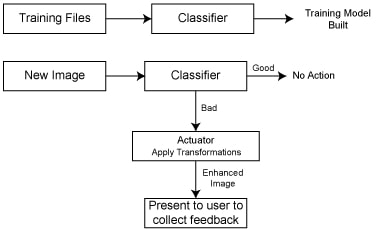
\includegraphics[scale=0.7]{Agent}
\end{figure}

\subsection{Environment}
The Environment class operated on a set of images captured by users under various lighting conditions (sunny, daylight, twilight, night ), scene types (portrait, landscape) and locations (indoor and outdoor). 
It presented the labelled images in the training set to the agent to build a model for classification.

\subsection{Sensor} 
A series of pre-processing steps such as cropping, scaling as well as feature extraction were performed automatically by the sensor to retrieve meaningful information so that our agent learns what a "good" photo should look like. The following 8 features are used:
\begin{enumerate}
  \item Number of Faces
  \item Face Hue
  \item Face Brightness
  \item Face Smoothness
  \item Eye Brightness
  \item Percentage of image occupied by faces
  \item Global contrast
  \item Sharpness of image
\end{enumerate}

\subsection{Percepts}
The percepts are images to be classified and enhanced by the agent. Examples of good and bad images are shown in Fig 2-5.
\begin{figure}[H]
\centering
\caption{Bad image with faces not visible}
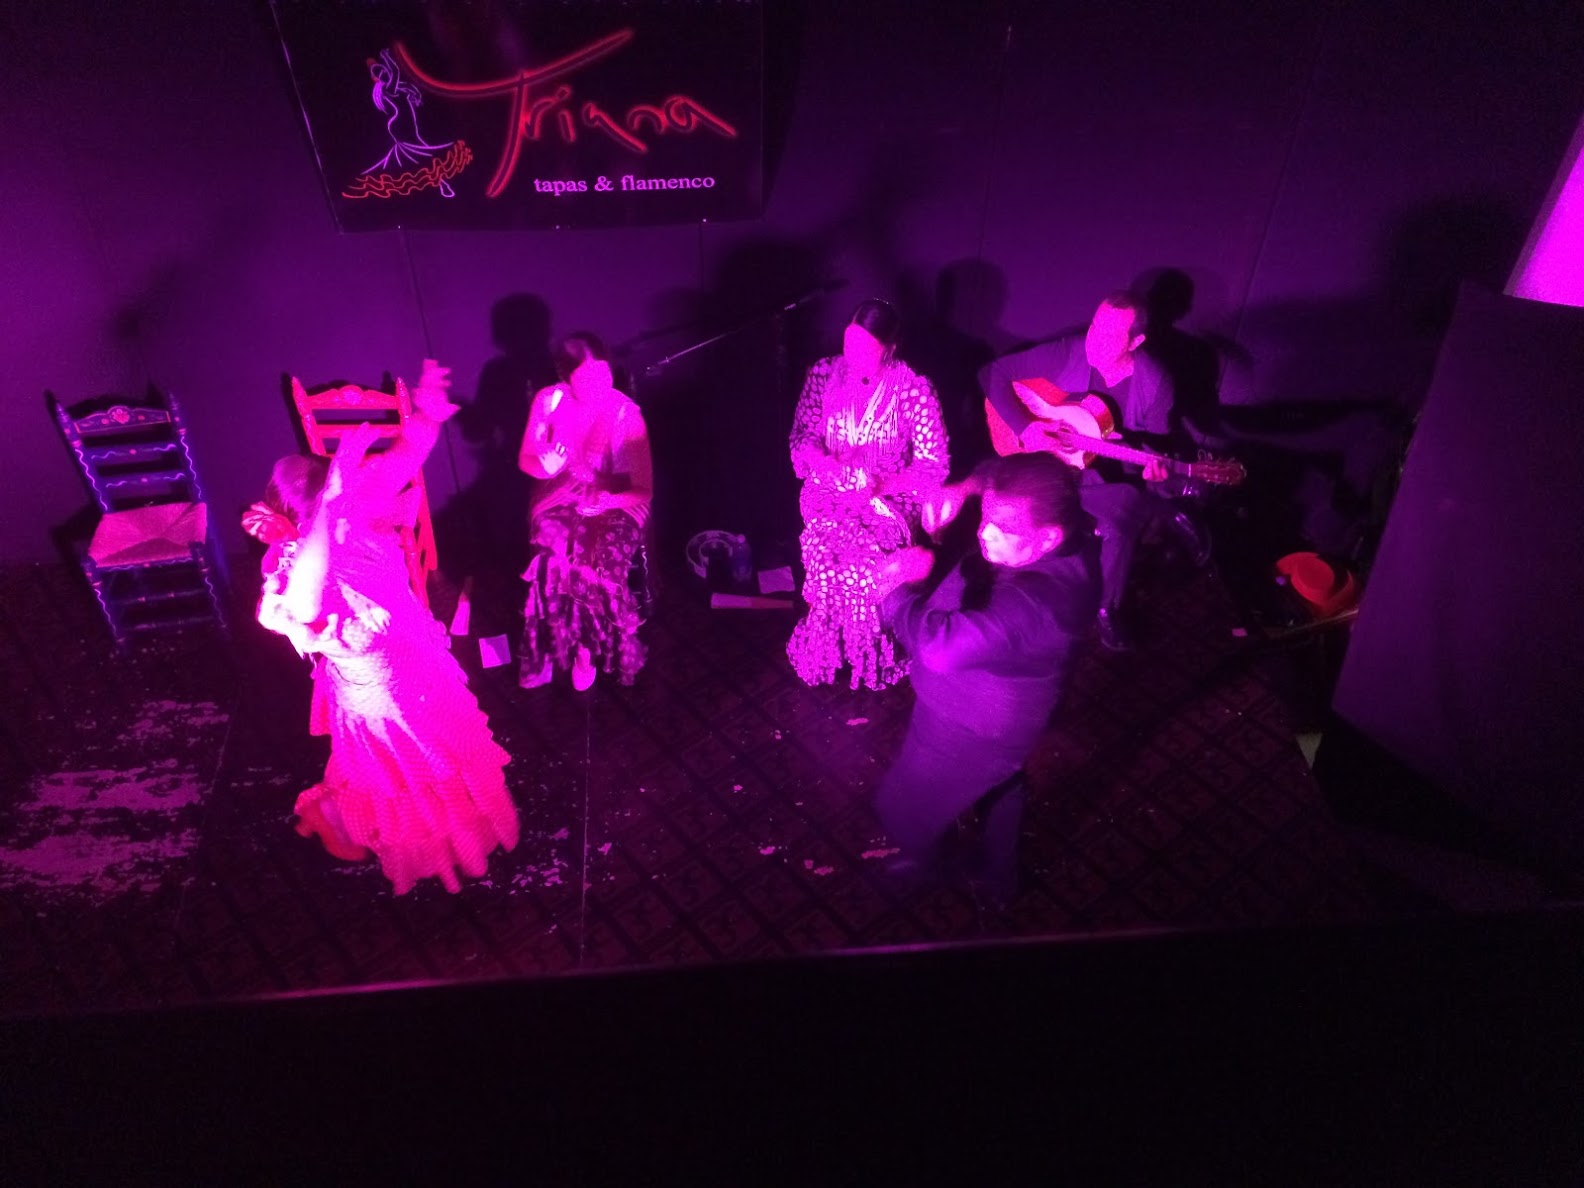
\includegraphics[scale=0.17]{0NoFaceDance}
\end{figure}

\begin{figure}[H]
\centering
\caption{Bad image with face not visible}
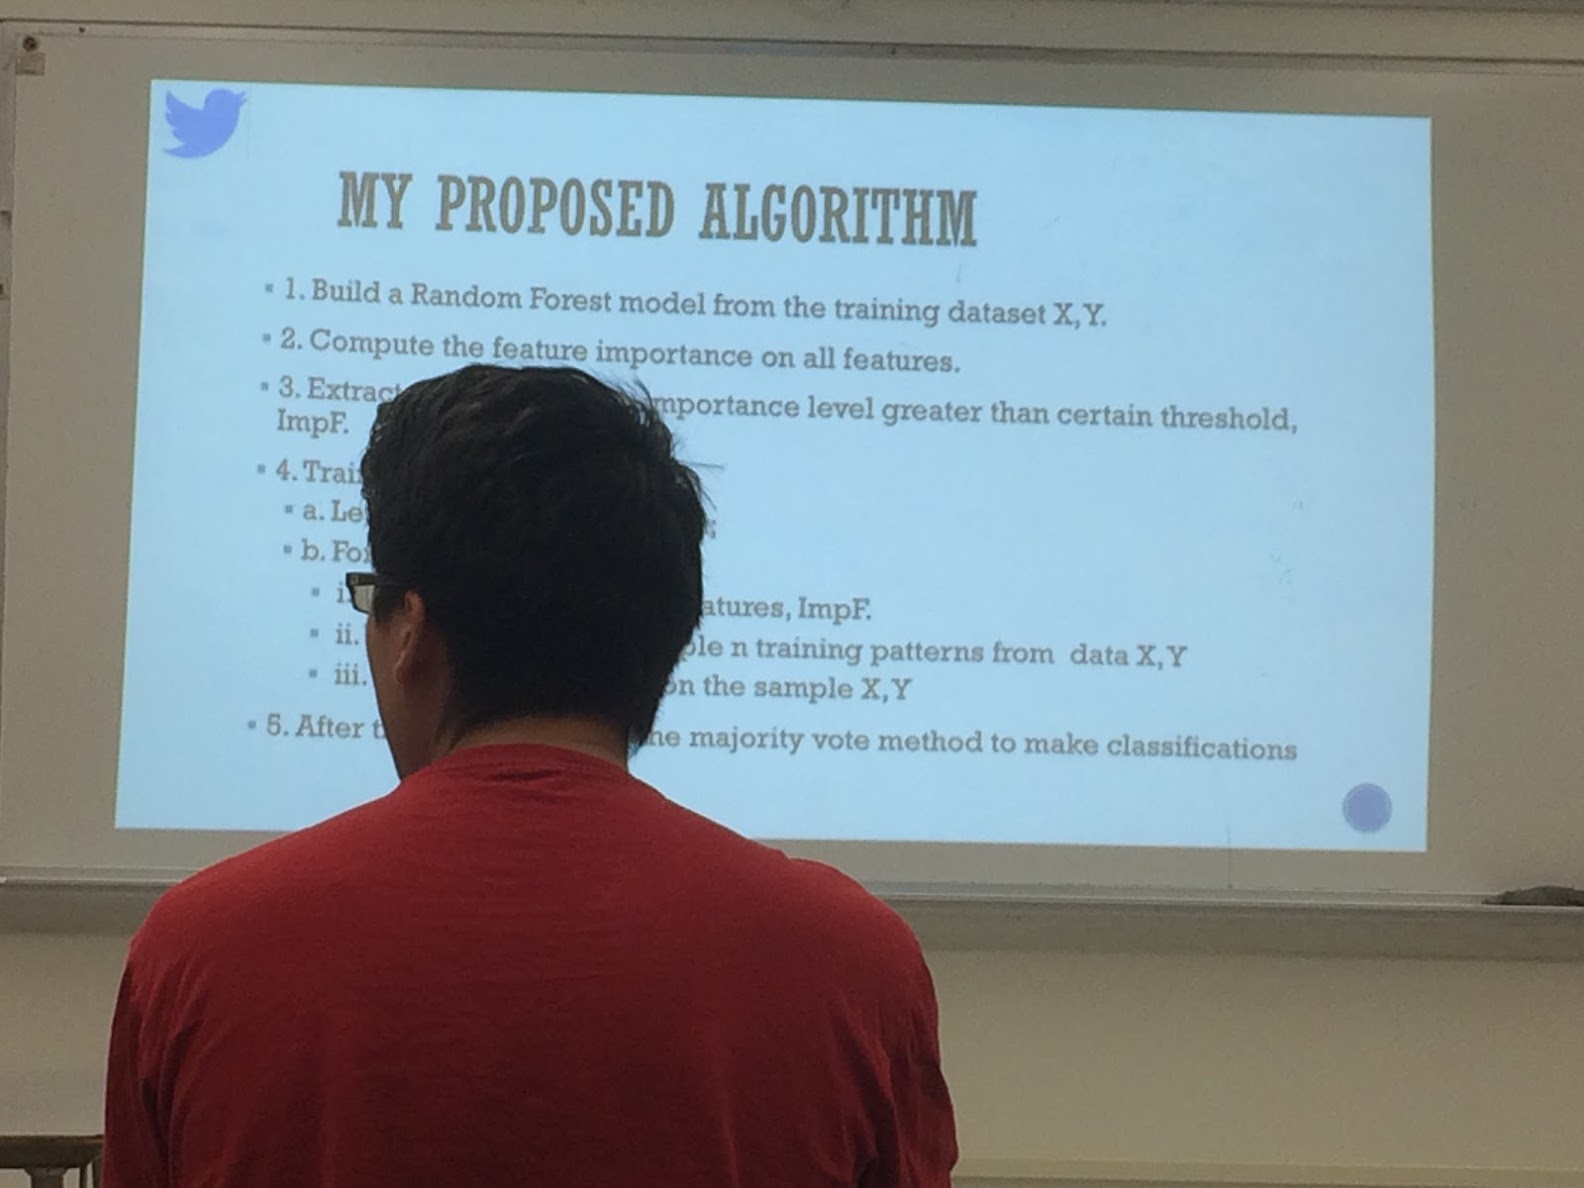
\includegraphics[scale=0.17]{BackHead}
\end{figure}

\begin{figure}[H]
\centering
\caption{Good Image}
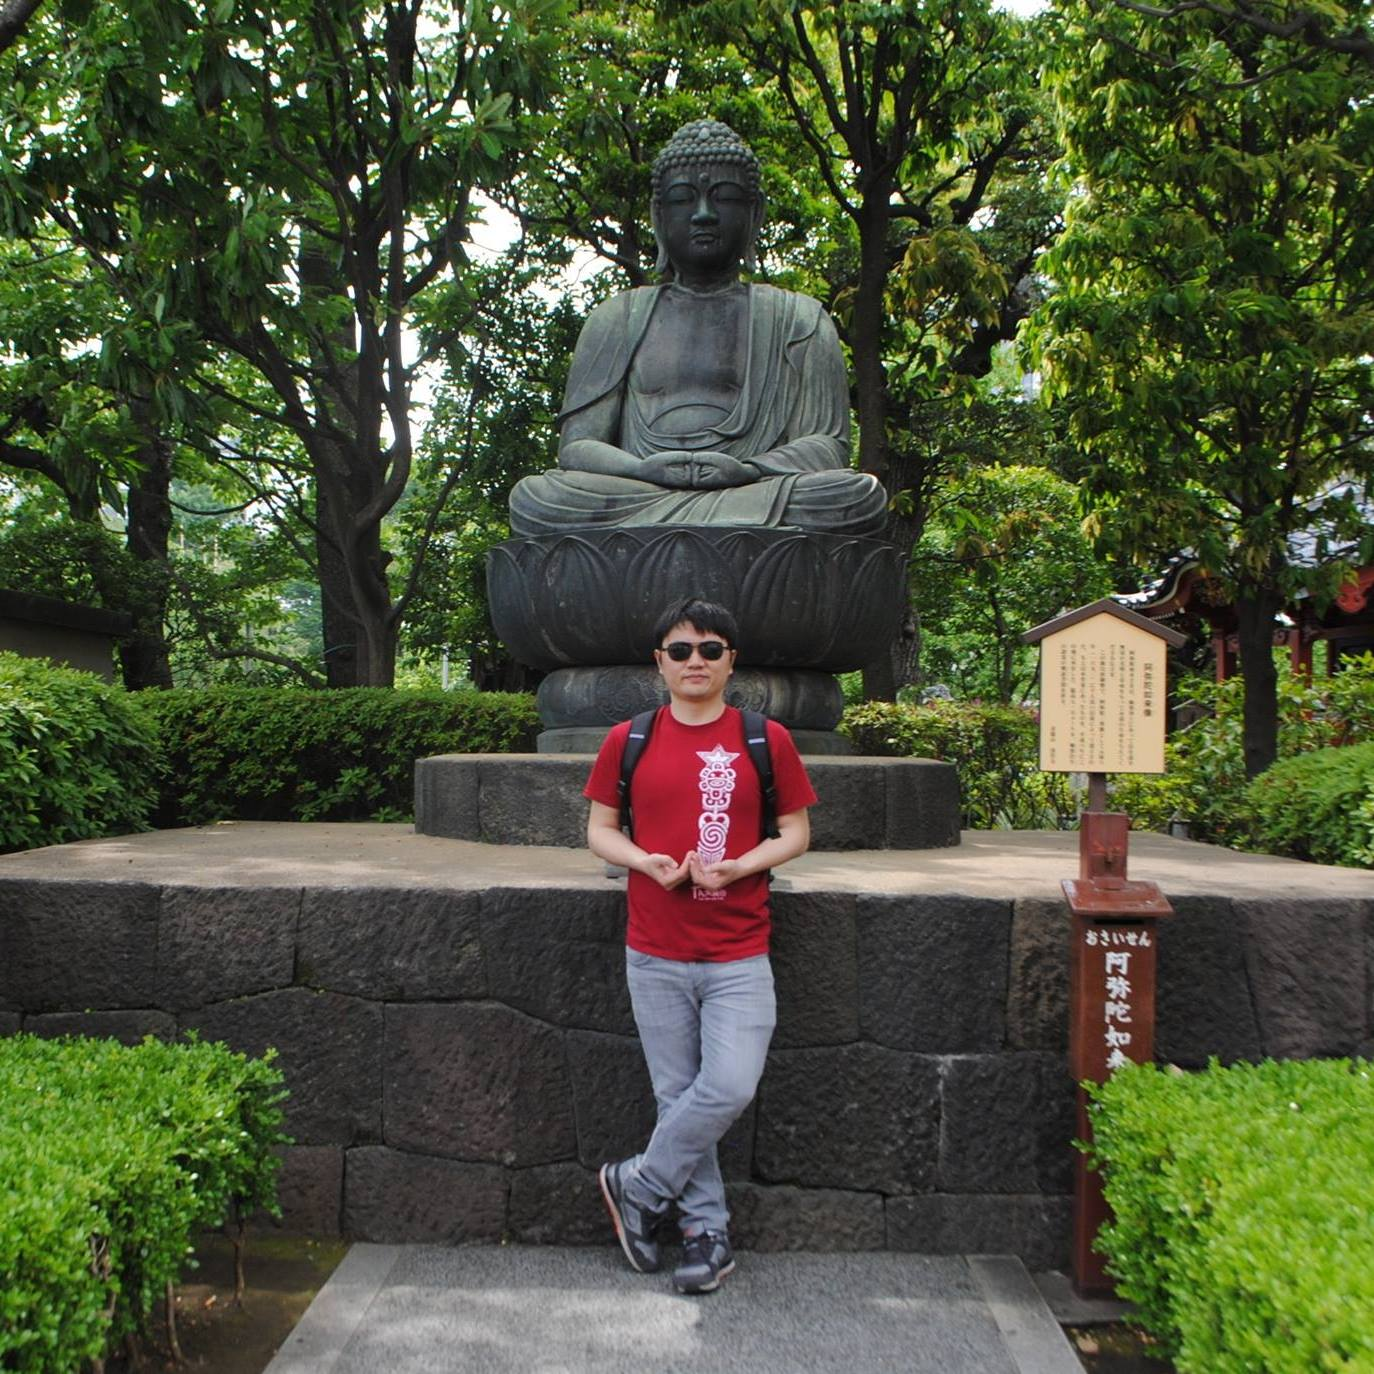
\includegraphics[scale=0.17]{JapanVisit}
\end{figure}

\begin{figure}[H]
\centering
\caption{Good Image}
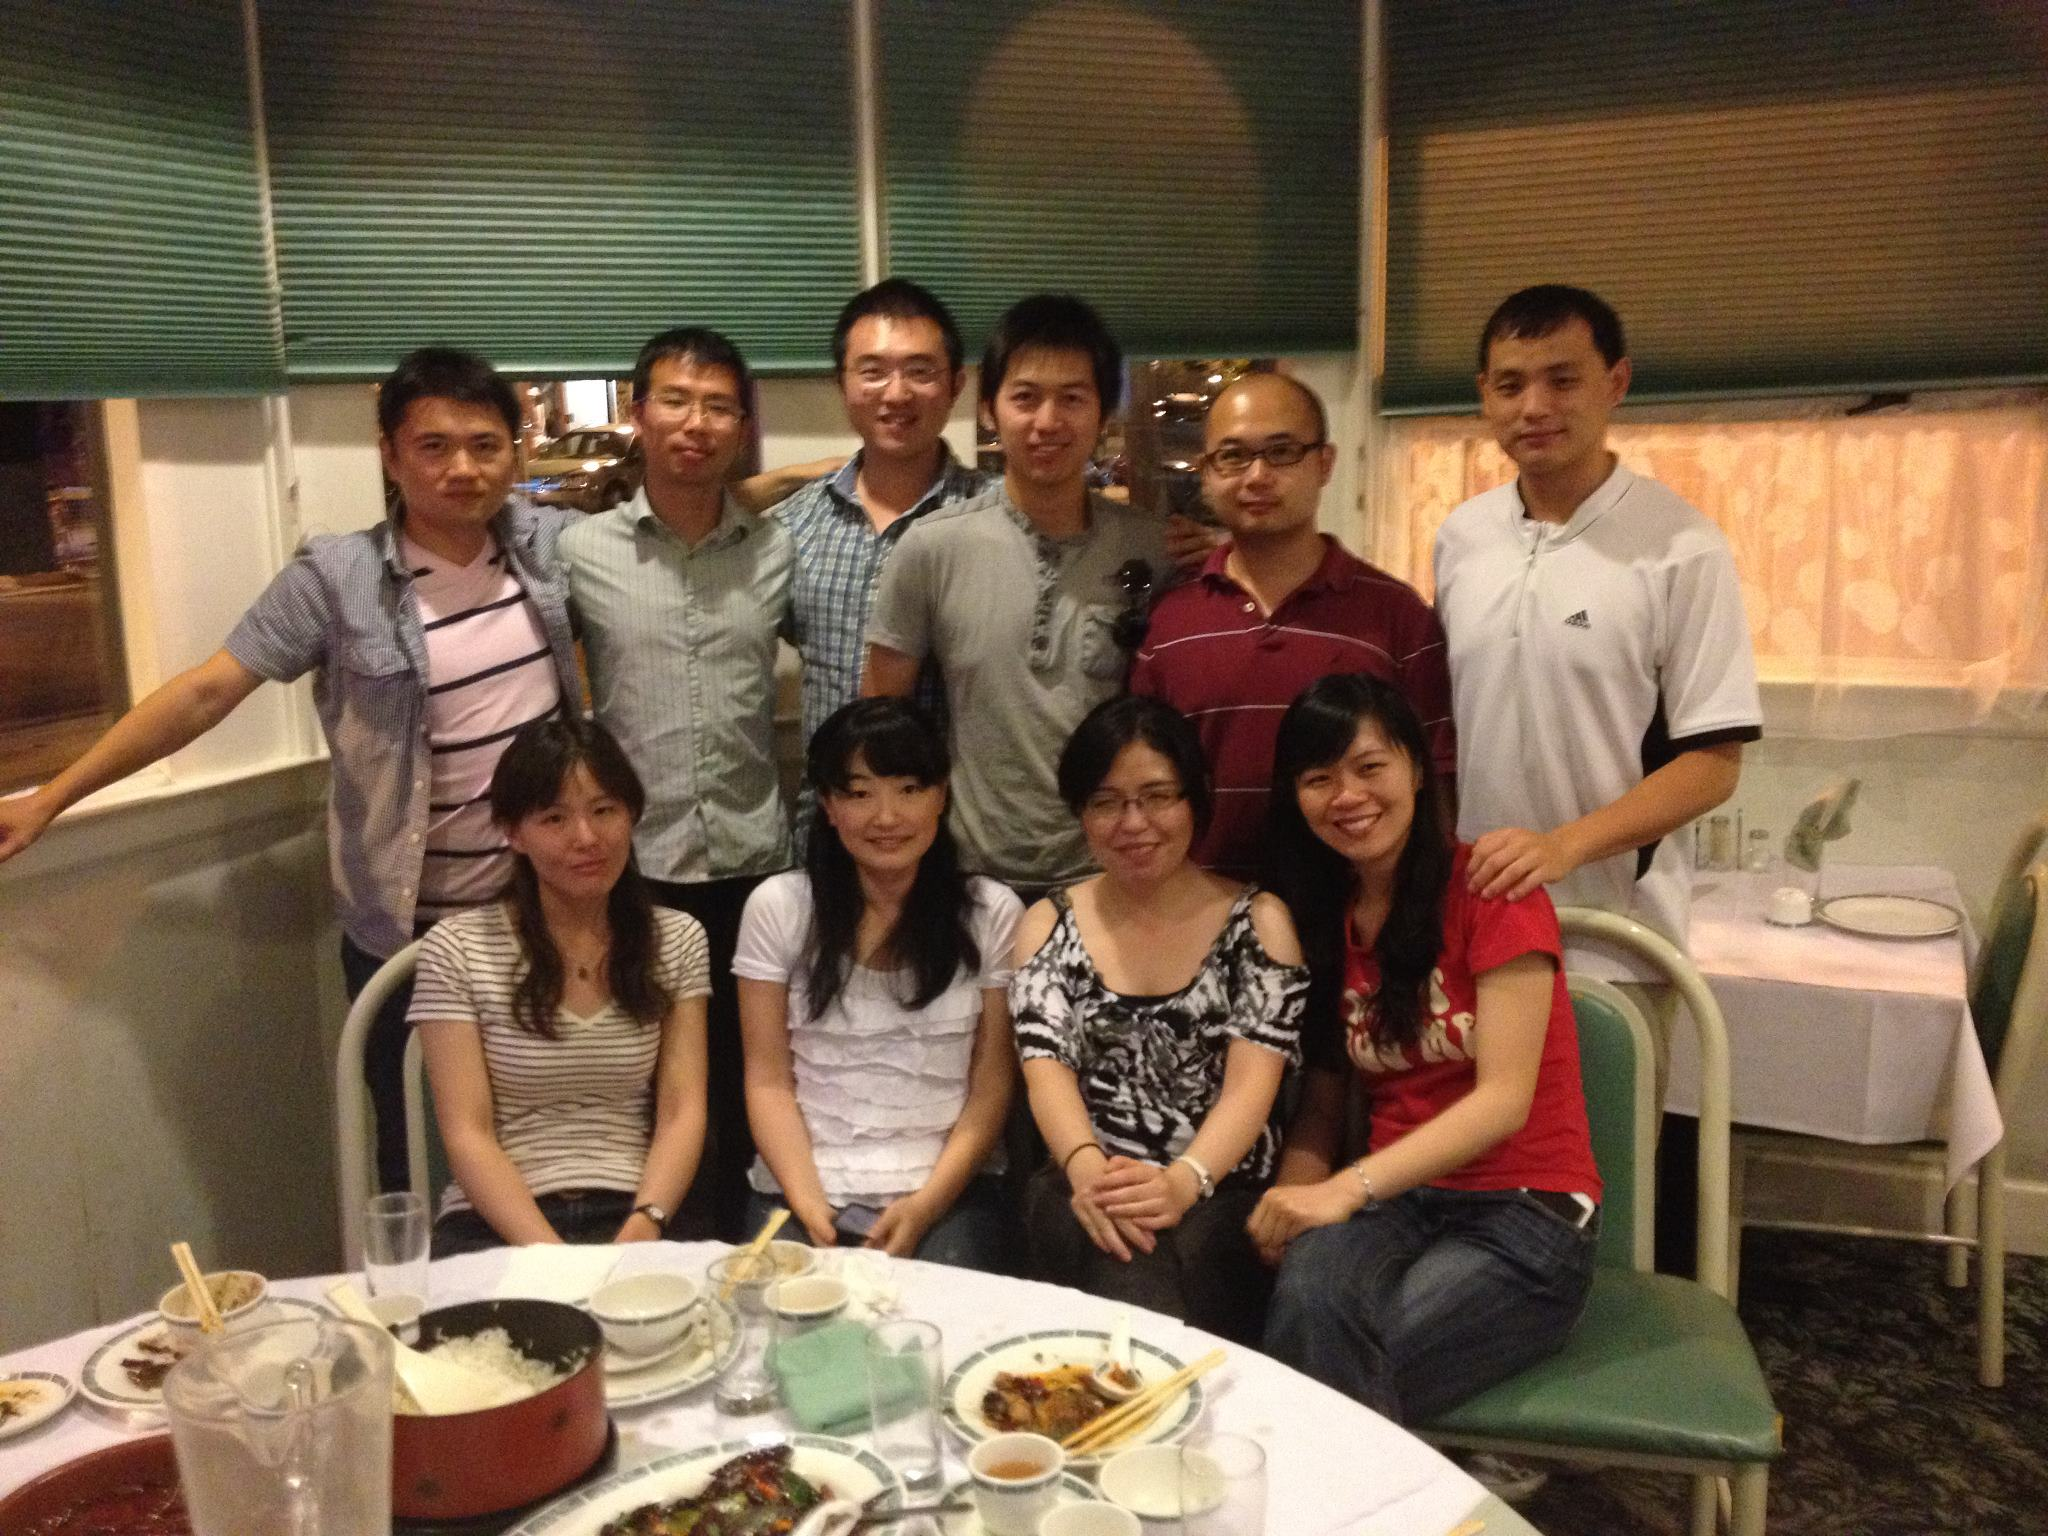
\includegraphics[scale=0.13]{Party2}
\end{figure}

\subsection{Agent Function}
The agent function classifies a perceived image as good or bad based on the classification model used (k-NN, SVM and Random Forest) and sends the result to the actuator. 
\subsection{Actuator}
The actuator enhances the image based on the classification result and sends it back to the Environment. 
\subsection{Performance Measures}
Our evaluation consists of two performance measures: 
\begin{enumerate}
  \item Comparison of original photo and agent-enhanced photo
  \item Comparison of agent-enhanced photo and photo enhanced automatically using third party software.
\end{enumerate}
The agent's performance is good if in both the above situations, the agent-enhanced photo is preferred by the user.
\section{Experiments}
\subsection{Training Data Set}
A training data set of 40 images was built manually and labelled "good" or "bad" based on our own personal taste. Since the agent is supposed to enhance photos based on the personal taste of individual users, a large number of photos are required to be stored for each user.
\subsection{Validation Data Set}
Validation data set was built using cross validation of the images in the dataset. 
\subsection{Test Data Set}
To assess the performance of our agent, we will obtain images of users from their social media accounts on Facebook and Instagram. Using the corresponding tag on these photos, these images will be labelled "good" or "bad" and then used for further testing.

\section{Results} 
\subsection{k Nearest Neighbors}
The k Nearest Neighbors classifier produced the following confusion matrix for k=5 with an accuracy of 64.10\%.
\begin{center}
 \begin{tabular}{||c c c||} 
 \hline\hline
Class & Predicted Good & Predicted Bad \\ 
 \hline
 Actual Good & 10 & 8\\
 \hline
 Actual Bad & 6 & 15\\
 \hline
\end{tabular}
\end{center}

\subsection{SVM}
The Support Vector Machine Classifier produced the following confusion matrix for linear kernel with an accuracy of 61.54\%.
\begin{center}
 \begin{tabular}{||c c c||} 
 \hline\hline
Class & Predicted Good & Predicted Bad \\ 
 \hline
 Actual Good & 8 & 10\\
 \hline
 Actual Bad & 5 & 16\\
 \hline
\end{tabular}
\end{center}

\subsection{Random Forest}
The Random Forest Classifier produced the following confusion matrix for 10 trees with an accuracy of 66.67\%.
\begin{center}
 \begin{tabular}{||c c c||} 
 \hline\hline
Class & Predicted Good & Predicted Bad \\ 
 \hline
 Actual Good & 11 & 7\\
 \hline
 Actual Bad & 6 & 15\\
 \hline
\end{tabular}
\end{center}

\subsection{Future Work}
Classes and modules to be implemented in the future are the actuator (photo enhancer) and performance measures. The following tasks need to be tackled in the next phase:
\begin{enumerate}
 \item  Collect more images for training model 
 \item  Enhance the image feature vector
  \item Find the parameters that give the best results for each classifier
  \item Implement photo enhancement based on the learning from the classification result.
  \item Implement performance measure of the enhancement by showing users the original, agent-enhanced and third party auto-enhanced image.
  \item Improve the user interface for labeling images in the dataset.
\end{enumerate}


\bibliography{AIProgressReport} 
\bibliographystyle{ieeetr}
\end{document}
































